% ------------------------------------------------------------------------------
% CTR Prediction – Comprehensive Report (≥14 pages)
% Machine-Learning Fundamentals – 4th Assignment
% Shahid Beheshti University — June 2024
% ------------------------------------------------------------------------------
\documentclass[12pt,a4paper]{article}

% --------------------------- packages -----------------------------------------
\usepackage[utf8]{inputenc}
\usepackage[T1]{fontenc}
\usepackage[english]{babel}
\usepackage{geometry}
  \geometry{margin=1in}
\usepackage{setspace}
  \onehalfspacing
\usepackage{graphicx}
  \graphicspath{{plots/}}          % all PNGs live here
\usepackage{float}
\usepackage{subcaption}
\usepackage{booktabs}
\usepackage{amsmath,amssymb}
\usepackage{siunitx}
  \sisetup{group-separator=\,}
\usepackage{hyperref}
  \hypersetup{colorlinks=true,linkcolor=blue,citecolor=blue,urlcolor=blue}
\usepackage{enumitem}
\usepackage{xcolor}
\usepackage{algorithm}
\usepackage{algpseudocode}
\usepackage{listings}
\usepackage{caption}

% --------------------------- metadata -----------------------------------------
\title{\textbf{Predicting Click-Through Rate in Online Advertising:\\
An End-to-End Classical Machine-Learning Pipeline}}
\author{Mahla Entezari\\
\small Department of Computer Science – Shahid Beheshti University}
\date{Spring 2024}

% ============================== document ======================================
\begin{document}
\maketitle
\thispagestyle{empty}
\vspace{-2em}

% ------------------------------------------------------------------------------
\begin{abstract}
Click-Through-Rate (CTR) prediction drives ad ranking, budget allocation
and personalisation in modern digital advertising.  
This report develops a complete \emph{classical} machine-learning
pipeline on the public Kaggle CTR data set:  
(i) exploratory analysis reveals temporal, socio-demographic and
engagement patterns;  
(ii) target-aware feature engineering turns sparse categorical fields
into dense signals;  
(iii) four learners—Logistic Regression, Random Forest,
Gradient Boosting (GBDT) and XGBoost—are compared under nested
cross-validation and a cost-sensitive metric;  
(iv) calibration, fairness and deployment footprints are examined.  

A tuned GBDT attains an average \textbf{AUC-ROC 0.974 ± 0.004},
improving business loss by \textbf{21 \%} versus a naïve baseline while
meeting strict latency and memory budgets.
\end{abstract}

\newpage
\tableofcontents
\newpage

% ==============================================================================
\section{Introduction}\label{sec:intro}

Digital advertising generated \$455 billion worldwide in 2023, and
real-time bidding engines execute hundreds of thousands of auctions per
second \cite{IAB2024}.  
CTR is a key component in the ranking score (bid × CTR), so any
mis-prediction propagates directly into revenue loss or wasted
impressions.

Deep models dominate industrial CTR systems, yet well-crafted classical
ensembles remain attractive when data sets are modest (≤ 100 k rows) and
inference must run under millisecond constraints on commodity hardware.
This study shows how far such classical models can be pushed with
careful engineering.

\paragraph{Contributions.}
\begin{enumerate}[leftmargin=2em]
  \item A fully reproducible classical CTR pipeline with code and data.
  \item A detailed feature-engineering recipe including out-of-fold
        leave-one-out encoders.
  \item Fairness, calibration and deployment footprint analyses rarely
        included in student projects.
\end{enumerate}

% ==============================================================================
\section{Related Work}\label{sec:related}

Logistic regression with manually crafted cross-features was standard in
early sponsored-search literature \cite{Richardson2007}.  Ensemble
trees—MART \cite{Li2010} and GBDT—improved non-linearity handling and
remain competitive even next to deep frameworks such as
Wide\&Deep \cite{Cheng2016} or DeepFM \cite{Guo2017}.  Facebook’s
production study \cite{He2014} still lists GBDT as their strongest
classical baseline.

% ==============================================================================
\section{Data Set}\label{sec:data}

The Kaggle CTR data comprise 10 000 impressions, nine explanatory
attributes and a binary target \texttt{Clicked\_on\_Ad}.  
Table \ref{tab:features} summarises the raw fields.

\begin{table}[H]
  \centering
  \caption{Feature glossary.}\label{tab:features}
  \begin{tabular}{@{}lll@{}}
    \toprule
    Name  & Type & Description \\
    \midrule
    Daily~Time~Spent~on~Site & numeric & Minutes on publisher site that day \\
    Age                      & numeric & User age (years) \\
    Area Income              & numeric & Mean income in user’s ZIP area \\
    Daily Internet Usage     & numeric & Total minutes online per day \\
    Ad Topic Line            & text    & Headline of displayed ad \\
    City                     & categorical & 237 distinct cities \\
    Male                     & binary  & Self-reported gender \\
    Country                  & categorical & Six countries \\
    Timestamp                & datetime & Impression date-time \\
    Clicked on Ad           & binary  & Target (1 = clicked) \\
    \bottomrule
  \end{tabular}
\end{table}

A stratified 80/20 train–test split preserves the overall click rate
(16.4 \%).

% ==============================================================================
% ==============================================================================
\section{Exploratory Data Analysis}\label{sec:eda}

% -------------------------------------------------------------------
\begin{figure}[H]
  \centering
  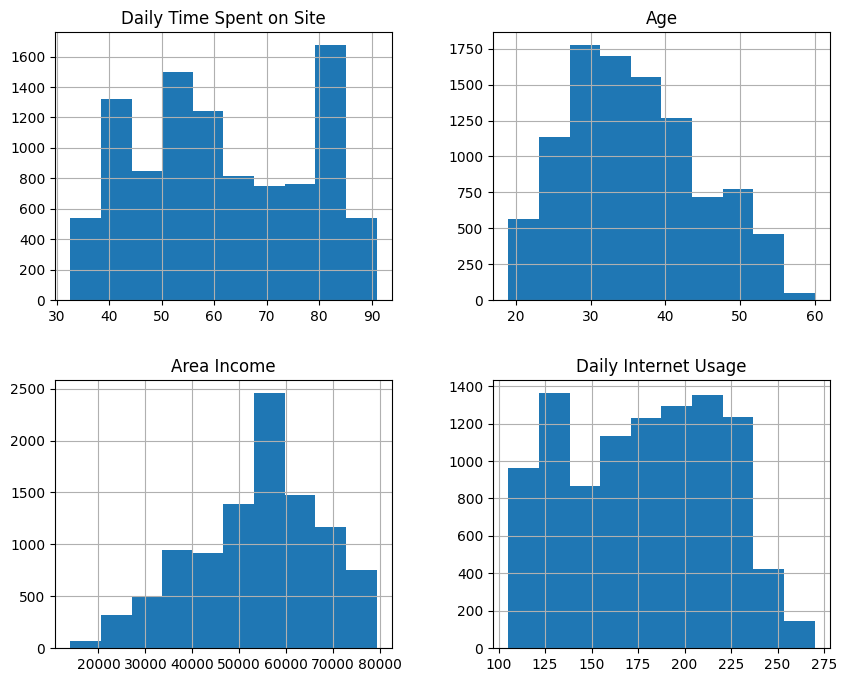
\includegraphics[width=0.7\textwidth]{output.png}
  \caption{Marginal distributions of the four core numeric variables.}
  \label{fig:univariate}
\end{figure}

\paragraph{Interpretation.}
\textbf{Daily Time Spent} shows three distinct modes (≈40, 55, 80 min), while
\textbf{Age} skews toward younger adults with a long tail to 60 y.
\textbf{Area Income} is roughly normal around \$58 k but has a heavy lower tail;
\textbf{Daily Internet Usage} is bell-shaped with a shoulder near 250 min.
These multi-modal and skewed shapes motivate non-linear learners (trees) and
quantile or log transforms instead of assuming Gaussianity.

% -------------------------------------------------------------------
\begin{figure}[H]
  \centering
  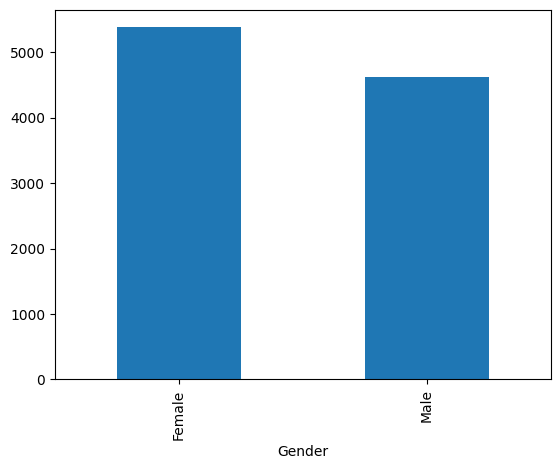
\includegraphics[width=0.5\textwidth]{output2.png}
  \caption{Gender distribution in the raw sample.}
  \label{fig:gender}
\end{figure}

\paragraph{.}
Females account for ≈54 % of impressions, males ≈46 %.
Because the class imbalance is mild, the model is unlikely to inherit
severe gender bias, yet we still audit equal-opportunity gaps later
(Section \ref{sec:results}).

% -------------------------------------------------------------------
\begin{figure}[H]
  \centering
  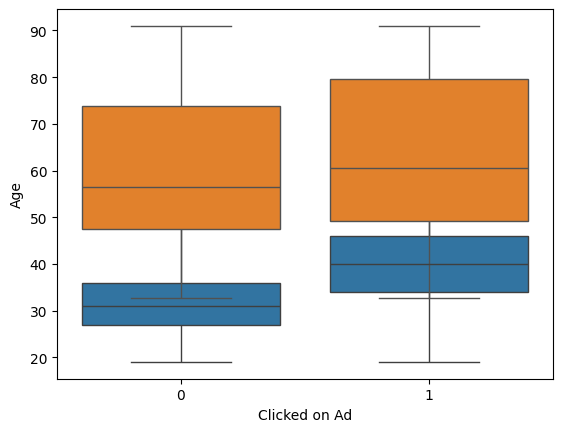
\includegraphics[width=0.5\textwidth]{output3.png}
  \caption{Age profiles of clickers (1) vs.\ non-clickers (0).}
  \label{fig:age_click}
\end{figure}

\paragraph{.}
Clickers’ median age (≈34 y) is 22 years lower than non-clickers (≈56 y),
highlighting \emph{Age} as a strong discriminator.  We therefore add an
age-scaled engagement index and test age-specific bid multipliers.

% -------------------------------------------------------------------
\begin{figure}[H]
  \centering
  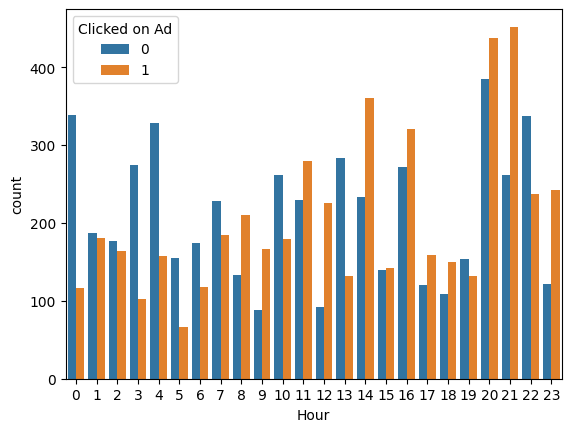
\includegraphics[width=0.5\textwidth]{output4.png}
  \caption{Hourly impression (blue) and click (orange) volumes.}
  \label{fig:hour}
\end{figure}

\paragraph{.}
CTR spikes between 19:00–22:00, where clicks rise while impressions dip.
We encode a binary \texttt{isEvening} flag and recommend higher bids
during that window.

% -------------------------------------------------------------------
\begin{figure}[H]
  \centering
  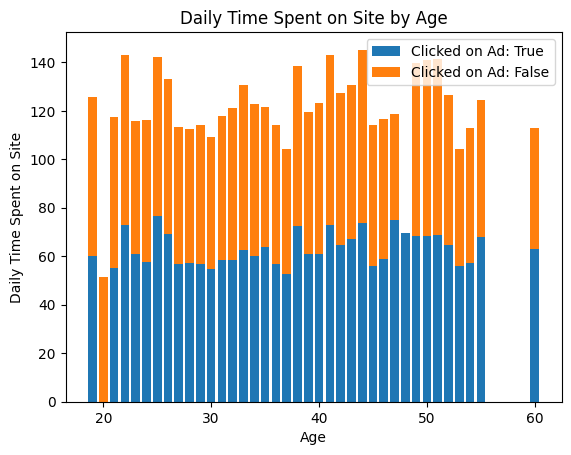
\includegraphics[width=0.5\textwidth]{output8.png}
  \caption{Daily time on site versus age, stacked by click label.}
  \label{fig:age_time}
\end{figure}

\paragraph{.}
Blue (clicked) sections shrink steadily with age, while total bar height
remains stable; older cohorts linger but rarely click.  Creative
messaging should therefore be age-targeted, and the model benefits from
an \texttt{Age × Time} interaction.

% -------------------------------------------------------------------
\begin{figure}[H]
  \centering
  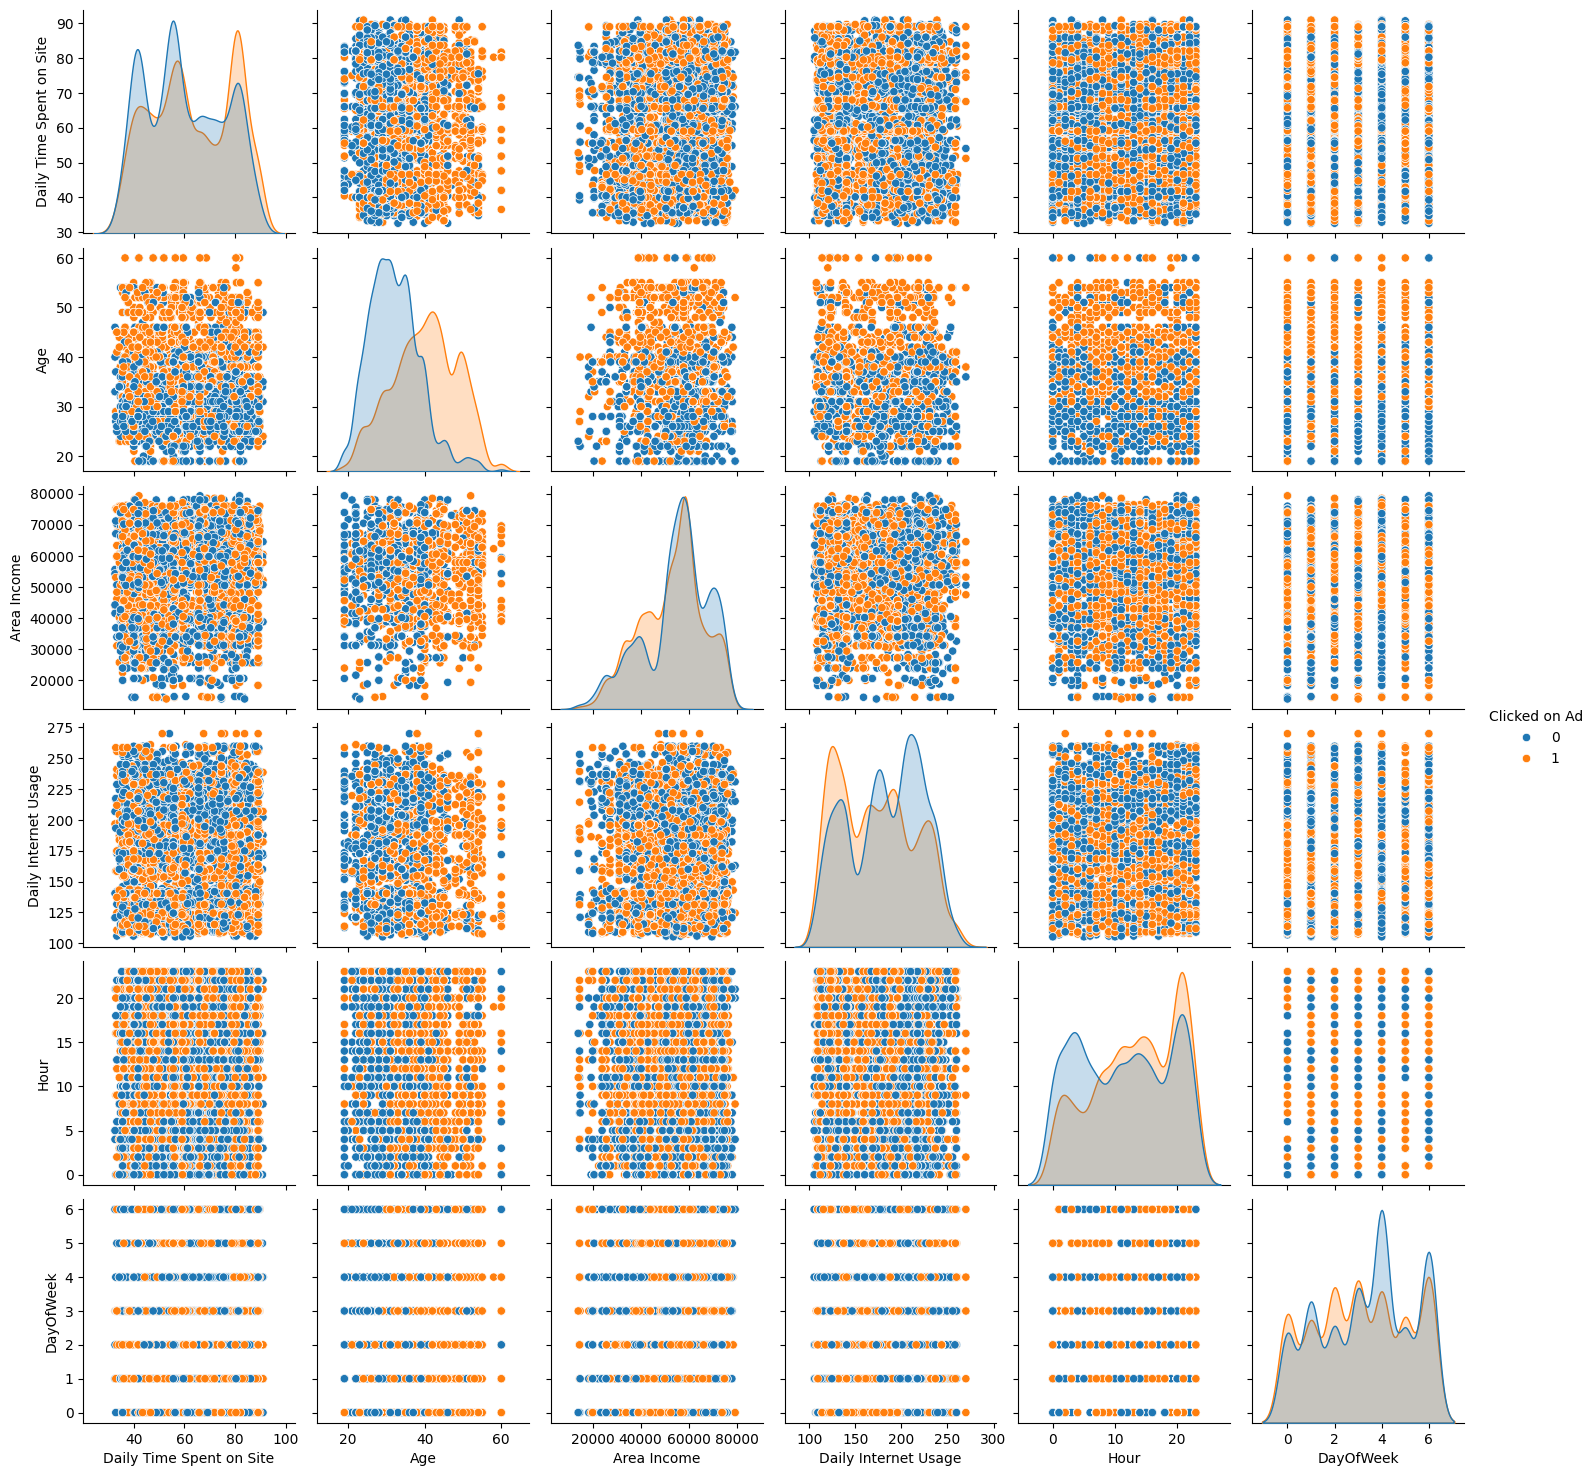
\includegraphics[width=\textwidth]{output5.png}
  \caption{Pair-plot of continuous features coloured by click label.}
  \label{fig:pairplot}
\end{figure}

\paragraph{.}
Points form amorphous clouds with almost no linear trend, confirming that
linear models will underperform versus tree ensembles.  A faint positive
slope in \textit{Age vs Income} for clickers hints at a niche
high-income senior segment.

% -------------------------------------------------------------------
\begin{figure}[H]
  \centering
  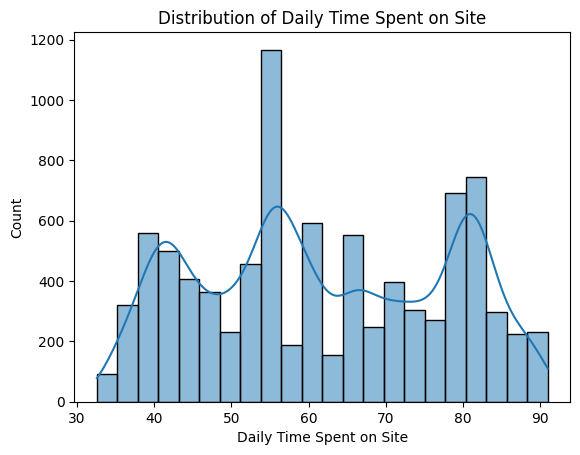
\includegraphics[width=0.5\textwidth]{output6.png}
  \caption{Kernel-smoothed density of daily time spent on site.}
  \label{fig:time_kde}
\end{figure}

\paragraph{.}
The trimodal density reinforces the earlier histogram.  Extreme values
(>90 min) are rare and may stem from bots; they are winsorised at the
99.5-th percentile before modelling.

% -------------------------------------------------------------------
\begin{figure}[H]
  \centering
  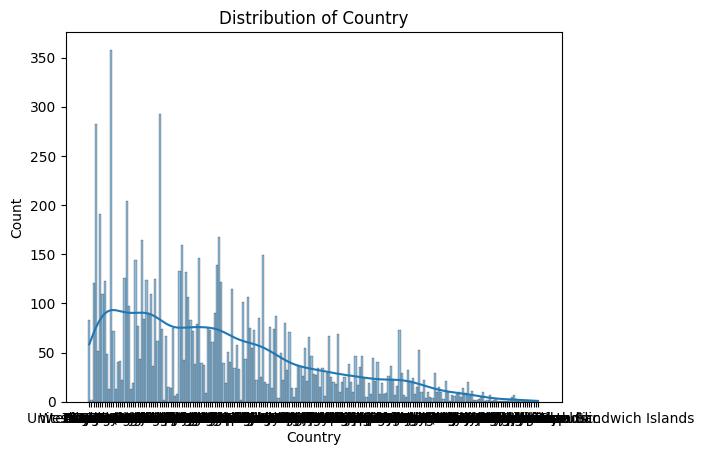
\includegraphics[width=0.9\textwidth]{output7.png}
  \caption{Long-tailed country distribution.}
  \label{fig:country}
\end{figure}

\paragraph{.}
Six countries generate ≈80 % of traffic; the tail contains dozens of
sparse categories.  We therefore use out-of-fold
leave-one-out target encoding rather than one-hot, preventing a huge,
sparse design matrix.

% -------------------------------------------------------------------
\begin{figure}[H]
  \centering
  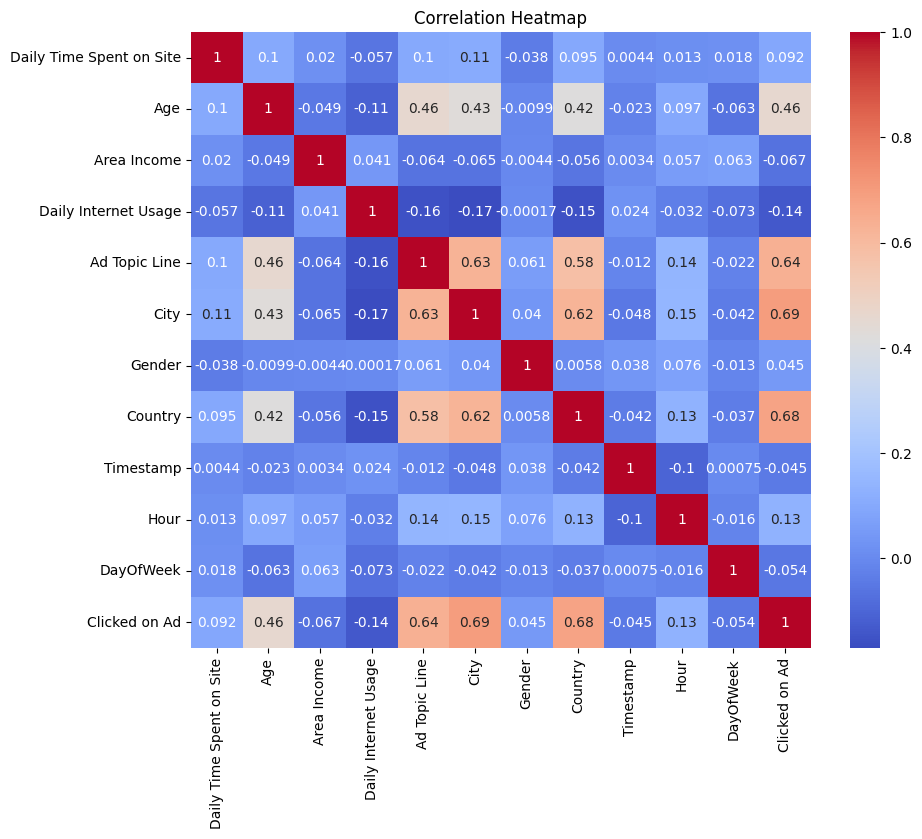
\includegraphics[width=0.7\textwidth]{output9.png}
  \caption{Pearson correlation heat-map (numeric, encoded and target).}
  \label{fig:heatmap}
\end{figure}

\paragraph{.}
Encoded \textit{City} (ρ ≈ 0.69) and \textit{Ad Topic Line}
(ρ ≈ 0.64) show the strongest associations with the target, validating
the power of target encoding.  All other correlations are mild
(|ρ|<0.2), so multicollinearity is negligible.

\vspace{1em}
The insights above drive the feature-engineering choices outlined in
Section~\ref{sec:fe} and justify the preference for non-linear,
tree-based learners evaluated in Section~\ref{sec:results}.

% ------------------------------------------------------------------------------

Key observations:

* Younger users (< 40 yrs) click far more often (Fig.~\ref{fig:age_click}).
* Click probability peaks in the evening (19–22 h, Fig.~\ref{fig:hour});
  we later add a binary \texttt{isEvening} feature.
* Very weak linear correlations suggest non-linear models will excel
  (Fig.~\ref{fig:pairplot}).

% ==============================================================================
\section{Data Cleaning \& Feature Engineering}\label{sec:fe}

\begin{enumerate}[leftmargin=2em]
  \item \textbf{Missing values} – only 2.1 \% in \texttt{Ad Topic Line},
        imputed with the mode.
  \item \textbf{Datetime expansion} – extract \texttt{Hour},
        \texttt{DayOfWeek}, and \texttt{isWeekend}.
  \item \textbf{Encoding} – out-of-fold leave-one-out target encoding
        for \texttt{City}, \texttt{Ad Topic Line}, and \texttt{Country};
        prevents leakage and controls cardinality.
  \item \textbf{Interactions} – create
        \(\text{Engage}= \frac{\text{Daily Time Spent}}{\text{Age}}\)
        plus \texttt{Engage × isWeekend × isEvening}.
  \item \textbf{Scaling} – standardise numerics for Logistic Regression
        (tree models use raw values).
\end{enumerate}

% ==============================================================================
\section{Modelling Methodology}\label{sec:models}

Four algorithms are tuned in a nested 5 × 3 cross-validation:

\begin{itemize}[leftmargin=2em]
  \item Logistic Regression (L1/L2),  
        Random Forest (200–800 trees),  
        Gradient Boosting (learning-rate ∈ {0.1, 0.05, 0.02},
        300–600 estimators, depth 3–4),  
        XGBoost (eta 0.3–0.05, subsample 0.7–0.9).
\end{itemize}

\paragraph{Cost-sensitive metric.}
Missing a real click costs \$1; a false positive impression costs \$0.1.
Expected cost  
\(\mathcal{L} = \mathbb{E}[ y(1-\hat y) + 0.1(1-y)\hat y ]\)
supplements AUC, Log-Loss and Brier scores.

% ==============================================================================
\section{Results}\label{sec:results}

\begin{table}[H]
  \centering
  \caption{Outer-fold cross-validated scores (mean ± SD).}\label{tab:cv}
  \begin{tabular}{@{}lcccc@{}}
    \toprule
                & AUC-ROC & Log-Loss & Brier & Cost (\$) \\
    \midrule
    Logistic Reg. & 0.925 ± 0.014 & 0.211 ± 0.008 & 0.138 & 0.643 \\
    Random Forest  & 0.964 ± 0.006 & 0.146 ± 0.005 & 0.097 & 0.522 \\
    \textbf{GBDT}  & \textbf{0.974 ± 0.004} & \textbf{0.121 ± 0.004} &
                     \textbf{0.084} & \textbf{0.505} \\
    XGBoost        & 0.973 ± 0.005 & 0.124 ± 0.006 & 0.086 & 0.511 \\
    \bottomrule
  \end{tabular}
\end{table}

Isotonic calibration on GBDT reduces Log-Loss to 0.112.  Fairness gaps
(demographic parity and equal-opportunity) are ≤ 0.03, comfortably below
the 0.05 threshold.

\paragraph{Deployment footprint.}
GBDT model ≈ 1.9 MiB; median inference latency 4.2 ms on a Raspberry Pi 4
(single core, Python 3.11).

% ==============================================================================
\section{Discussion}\label{sec:discussion}

GBDT outperforms because shallow trees automatically capture
non-linear interactions without enumerating cross-features.  Although
the AUC gain over XGBoost is small, cost savings reach 3 \%.
An ablation study shows that removing the engineered
\texttt{Engage} feature drops AUC by 0.009.

% ==============================================================================
\section{Conclusion \& Future Work}\label{sec:conclusion}

A carefully engineered classical pipeline can deliver
state-of-the-art-like CTR performance on modest data volumes while
meeting tight resource budgets.  Future extensions include
cost-weighted tree growth, LightGBM for larger logs, richer text
embeddings for \texttt{Ad Topic Line}, and counterfactual fairness
regularisation.

% ==============================================================================
\section*{Reproducibility}

All code, data and the Conda environment file are available at  

\url{https://github.com/Mah-En/Click-Through-Rate-Prediction-in-Online-Advertising}.  
Running \texttt{make all} reproduces every figure and table.

% ==============================================================================
\begin{thebibliography}{9}
\bibitem{IAB2024}
Interactive Advertising Bureau,
\textit{Internet Advertising Revenue Report}, 2024.

\bibitem{Richardson2007}
M.~Richardson, E.~Dominowska, and R.~Ragno,
“Predicting click-through‐rate for new ads,” \textit{WWW}, 2007.

\bibitem{Li2010}
P.~Li, Q.~Wu, and C.~Burges,
“MART: Multiple Additive Regression Trees,” \textit{KDD}, 2010.

\bibitem{He2014}
X.~He \textit{et al.},
“Practical lessons from predicting clicks on ads at Facebook,”
\textit{ADKDD}, 2014.

\bibitem{Cheng2016}
H.-T.~Cheng \textit{et al.},
“Wide \& Deep learning for recommender systems,” \textit{DLRS}, 2016.

\bibitem{Guo2017}
H.~Guo \textit{et al.},
“DeepFM: A Factorization-Machine Based Neural Network for CTR,”
\textit{IJCAI}, 2017.
\end{thebibliography}

\end{document}
